\textbf{Date:} June 6th 2014\\\textbf{Duration:} 11-13\\\textbf{Group
members:} Henrik

\subsection{Goals for today}

\begin{itemize}
\item
  Discover solar panels and their states (color)
\item
  Make the robot align with the line nicely so it may hit the solar
  panels correctly
\item
  Create a testing program using hard coded values and experiment with
  this
\end{itemize}

\subsection{Discover solar panels}

In the previous session, we made quite a few measurements for the color
sensor when a red, blue or black solar panel was present (or none at
all). We made these measurements multiple times under different lighting
conditions. Based on this, we have found a way to discover the different
states the solar panels may be in.

\begin{figure}[h]
  \centering
  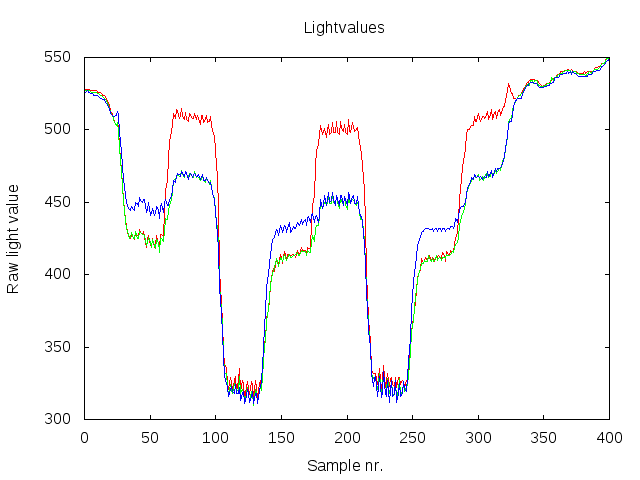
\includegraphics[scale=0.342]{../experiments/2prototype/results/gnuplot/Colormesrun1.png}
  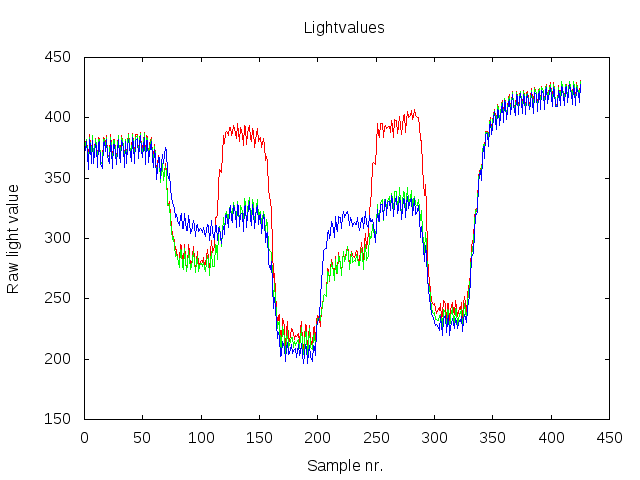
\includegraphics[scale=0.342]{../experiments/2prototype/results/gnuplot/Colormesrun2.png}
  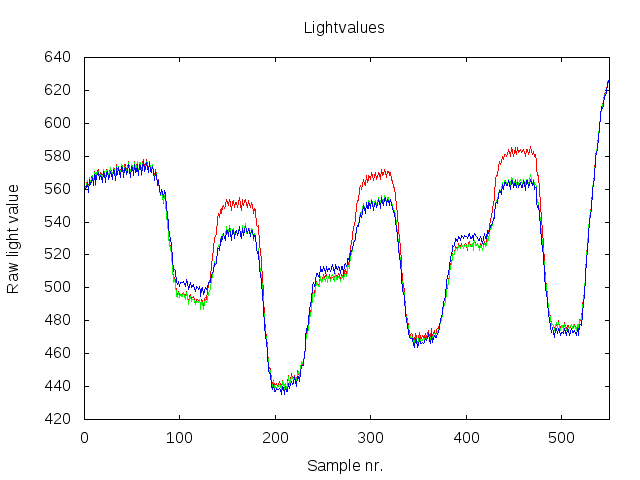
\includegraphics[scale=0.34]{../experiments/2prototype/results/gnuplot/Colormesrun3.png}
  \caption{Three color mesurements when the robot drives over 8 solarpannels in a
straight line (none,blue,red,black,blue,red,black,blue,red,none)}
\end{figure}

\subsubsection{First idea for discovering solar panels}
On every graph, it is clear that all the RGB-values are high when no
solar panel is present, but when a panel is present, the values change.
When a solar panel is present, we see on our measurements that the green
value is always among the lowest, so we are going to make a function
that takes the value when there is no solar panel (ValueNone) and
subtracts the value for green (ValueGreen) and checks whether the
difference is large enough to determine whether a solar panel is
present.


\begin{longtable}[c]{|l|c|c|c|l|c|c|}
\hline
Detection color & 
\multicolumn{3}{c|}{Mesured values for the three runs} &
\multicolumn{3}{c|}{equal to this offset}\\\hline 
Blue (max-green) & 525-425 & 375-275 & 570-490 &= 100 & 100 & 80 \\
Red (max-green)  & 525-475 & 375-325 & 570-530 &=  50 &  50 & 40 \\
Black (max-green)& 525-325 & 375-225 & 570-450 &= 200 & 150 &120\\
\hline
\caption{Measurement for the three graphs.}
\end{longtable}


As can be seen in the calculations above, red is very difficult to
discover as the difference needs to be greater than 39 (approximately),
and this was also reflected in the test run we made using these
calculations.

\subsubsection{Second idea for discovering solar panels}

The values for when there is no solar panel present (ValueNone) are all
very large and there is very little difference between them. We are
going try to incorporate this, so that when the RGB-values become very
small, but the difference between them is still very small, we can
conclude it is a black solar panel. In the same way, when the difference
between them is large, it is either a red or a blue solar panel; if the value between blue and green is small then it is a red solar panel, and finally, if the value between red and green is small then it is a blue solar panel.

This approach has worked on 2-3 tests for each color, so we are
satisfied with this idea at the moment.

\subsection{Hitting the solar panels correctly}

We have a problem with the robot's direction being a bit off when the
last turn has been made (when it should be on the line with three solar
panels in front of it. The back wheel is not aligned with the track, so
even though we are using a P-controller to control the direction of the
front of the robot, it will always be a bit off, and as a consequence,
we will ``always'' hit the solar panels a bit off. As such, we need to
align the robot before we can attempt to pick up a solar panel.

\subsubsection{First idea}

Drive straight forwards and backwards until the backside light sensor
hits exactly on the darkest part of the line we want to follow, then
turn the front part of the robot onto the line also. In connection with
this, we need to consider whether the front light sensor needs to be
centered with regards to the robot or whether it should continue to be
aligned a bit to the left side of the robot.

\subsection{Conclusion}

We made a function for discovering solar panels that we are reasonably
satisfied with using the RGB-values from the color sensor. We started on
an idea for hitting the solar panels correctly, but did not finish. We
will continue with this in the next session.
